\documentclass{beamer}
\usepackage[orientation=portrait,size=A4,scale=3]{beamerposter}

\usepackage{etex}
\usepackage[utf8]{inputenc}
\usepackage[T1]{fontenc}
\usepackage[frenchb]{babel}
\usepackage{hyperref}
\usepackage{graphicx}
\usepackage{animate}
\usepackage{tikz}
\usepackage{pgfplots}

\DeclareUnicodeCharacter{00A0}{ }

\usetheme{Hannover}
\usecolortheme{orchid}

\title{Le problème SAT}
\subtitle{TIPE math}
\author{Luc Chabassier}
\institute{Lycée Pierre de Fermat}

\setbeamertemplate{itemize item}[ball]
\setbeamertemplate{itemize subitem}[triangle]
\setbeamertemplate{itemize subsubitem}[circle]
\setbeamertemplate{blocks}[rounded]

\begin{document}
\section{SAT}
\begin{frame}
    \maketitle
    \begin{block}{Définition}
        Problème de décision : recherche d'une valuation évaluant à vrai pour une formule booléenne.
    \end{block}

    \begin{exampleblock}{Exemple}
        \begin{itemize}
            \item UNSAT : $(x_0\vee x_1) \wedge (\neg x_0\vee x_1) \wedge (x_0\vee\neg x_1) \wedge (\neg x_0\vee\neg x_1)$
            \item SAT : ${\color{green}{\color{blue}x_0}\wedge\neg{\color{red}({\color{blue}x_0}\wedge\neg{\color{green}({\color{blue}x_1}\wedge\neg{\color{red}({\color{blue}x_1}\wedge {\color{orange}x_2})})})}}$
        \end{itemize}
    \end{exampleblock}
    \begin{exampleblock}{Applications}
        \begin{itemize}
            \item En cryptographie.
            \item En résolution de dépendances.
            \item En biologie.
        \end{itemize}
    \end{exampleblock}
    \begin{alertblock}{NP-Complet}
        Théorème de Cook (1971)
    \end{alertblock}
    \begin{exampleblock}{Forme normale conjonctive}
        $(h\vee\neg b) \wedge (e\vee\neg h\vee\neg c) \wedge (\neg g\vee\neg d\vee\neg c) \wedge (a\vee\neg h\vee d) \wedge (a\vee\neg d\vee\neg e\vee g)$
    \end{exampleblock}
    \begin{block}{NP-Complet}
        \[ \begin{array}{cl}
                & x_0 \wedge \neg(x_0 \wedge \neg(x_1 \wedge \neg (x_1 \wedge x_2))) \\
                \sim & x_0 \wedge (\neg x_0 \vee (x_1 \wedge (\neg x_1 \vee \neg x_2))) \\
                \sim & x_0 \wedge (\neg x_0 \vee a) \wedge (\neg x_1 \vee \neg x_2 \vee \neg a) \\
           \end{array}
        \]
    \end{block}
\end{frame}

\section{HIPP}
\begin{frame}
    \frametitle{Le problème HIPP}
    \begin{block}{Génome somme d'haplotypes}
            \[ \left(\begin{array}{c} 1 \\ 1 \\ 0 \end{array}\right) \bigoplus \left(\begin{array}{c} 1 \\ 0 \\ 0\end{array}\right) =
                \left(\begin{array}{c} 1 \\ 2 \\ 0 \end{array}\right) \]
    \end{block}
    \begin{block}{Objectif}
        Minimisation de l'ensemble d'haplotypes pour une population.
    \end{block}
    \begin{exampleblock}{Exemple}
        La population
        \[\begin{array}{c} \{(0,0,0,1),(1,0,0,1),(0,1,0,1), \\ (2,0,0,1),(0,2,0,1),(2,2,0,1)\}\end{array} \]
        peut se déduire des haplotypes
        \[\{(0,0,0,1),(1,0,0,1),(0,1,0,1)\}\]
    \end{exampleblock}

    \begin{block}{Conversion en SAT}
        Formule pour la population $\left\{(2, 0, 1))\right\}$ avec $2$ haplotypes.
        Variables : $h_k(j)$ pour $1\leq k\leq 2$ et $1\leq j\leq 3$, $s^a_i(k)$ et $s^b_1(k)$ pour $1\leq k\leq 2$ et $a_1$, $a_2$.
        \[
            \begin{array}{cl} & (s^a_1(1)\vee s^a_1(2)) \wedge (s^b_1(1)\vee s^b_1(2)) \\
                \wedge & (a_1 \vee a_2) \wedge (\neg a_1 \vee \neg a_2) \\
                \wedge & \left(\begin{array}{cl}
                                   & (\neg s^a_1(1) \vee a_1 \vee h_1(1)) \\
                            \wedge & (\neg s^a_1(1) \vee \neg a_1 \vee \neg h_1(1)) \\
                            \wedge & (\neg s^b_1(1) \vee a_2 \vee h_1(1)) \\
                            \wedge & (\neg s^b_1(1) \vee \neg a_2 \vee \neg h_1(1)) \\
                         \end{array}\right) \\
                \wedge & \left(\begin{array}{cl}
                                   & (\neg s^a_1(1) \vee a_1 \vee h_2(1)) \\
                            \wedge & (\neg s^a_1(1) \vee \neg a_1 \vee \neg h_2(1)) \\
                            \wedge & (\neg s^b_1(1) \vee a_2 \vee h_2(1)) \\
                            \wedge & (\neg s^b_1(1) \vee \neg a_2 \vee \neg h_2(1)) \\
                       \end{array}\right) \\
                \wedge & \left(\begin{array}{cl} & (\neg s^a_1(1) \vee \neg h_1(2)) \wedge (\neg s^b_1(1) \vee \neg h_1(2)) \\
                                    \wedge & (\neg s^a_1(2) \vee \neg h_2(2)) \wedge (\neg s^b_1(2) \vee \neg h_2(2)) \\
                         \end{array}\right) \\
                \wedge & \left(\begin{array}{cl} & (\neg s^a_1(1) \neg h_1(3)) \wedge (\neg s^b_1(1) \vee h_1(3)) \\
                                    \wedge & (\neg s^a_1(2) \vee h_2(3)) \wedge (\neg s^b_1(2) \vee h_2(3)) \\
                         \end{array}\right) \\
            \end{array}
        \]
    \end{block}

\end{frame}

\section{Algorithme}
\begin{frame}
    \frametitle{Algorithme CDCL}
    \begin{block}{Choix des variables}
        Espace de recherche : arbre binaire.
    \end{block}
    \begin{block}{DPLL}
        Assignation partielles testées.
    \end{block}
    \begin{center}
        \includegraphics[width=0.8\linewidth]{../reso/error.pdf} \\
        \vspace{1em}
        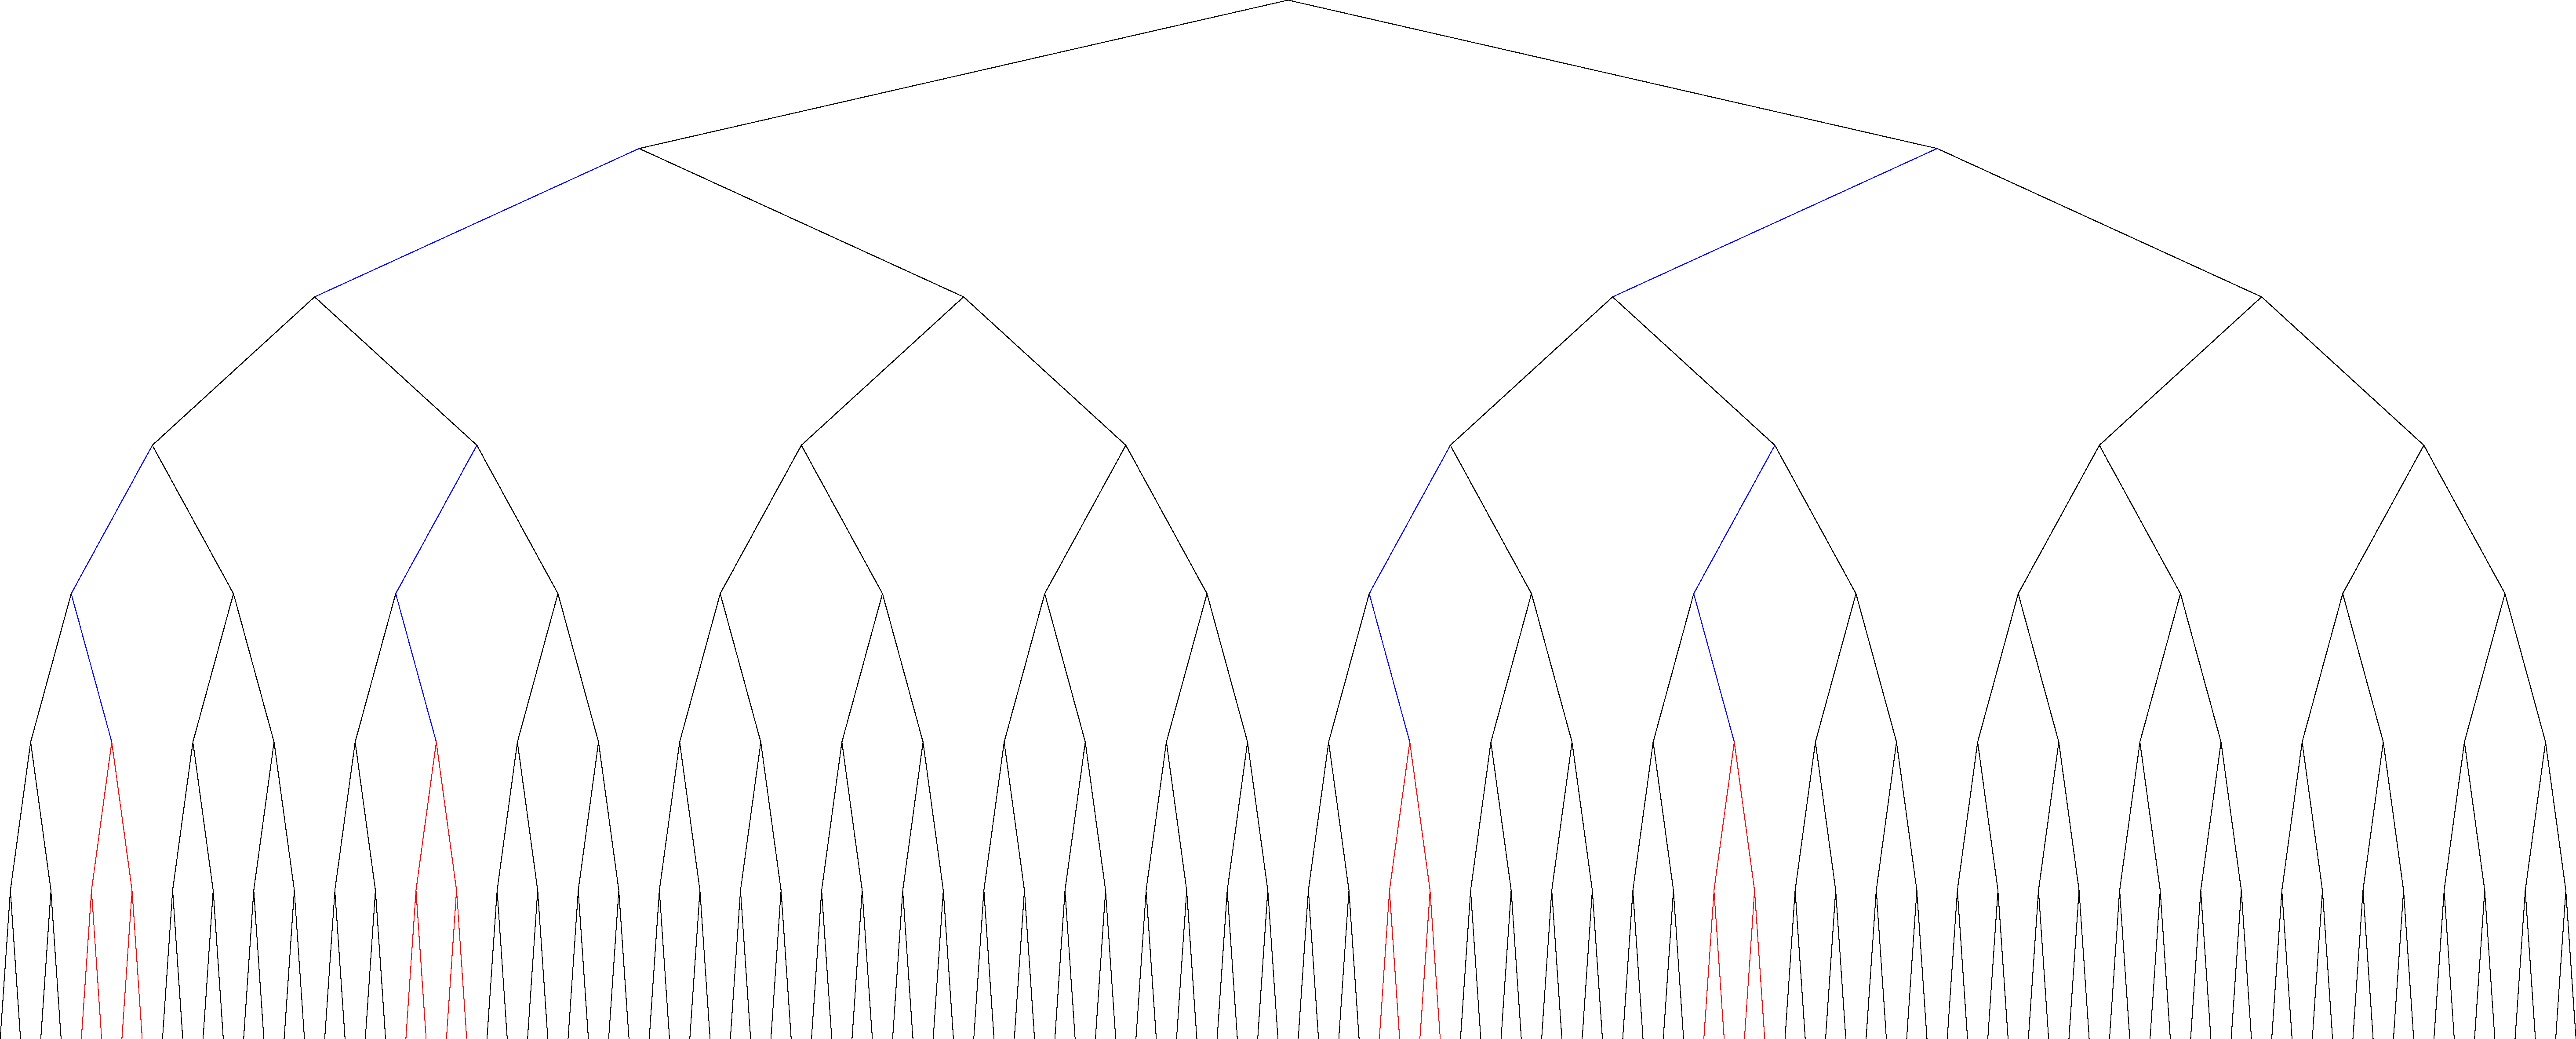
\includegraphics[width=0.8\linewidth]{../reso/eliminated.pdf}
    \end{center}
    \begin{block}{CDCL}
        \begin{itemize}
            \item Apprentissage de variables.
            \item Retour non chronologique.
        \end{itemize}
    \end{block}

    % Parler de l'heuristique VSIDS, non pure
    \begin{block}{Heuristiques dans le choix de la variable}
        Favoriser l'apparition des conflits.
    \end{block}

    % Gain de temps observé et meilleure stabilité
    % Mentionner stratégie géométrique et de Luby
    \begin{block}{Redémarrages}
        Stratégie de redémarrage : $(t_n)_{n\in\mathbb{N}}\in(\mathbb{N}^*)^\mathbb{N}$
    \end{block}

    \begin{exampleblock}{Application au problème HIPP}
        \begin{itemize}
            \item Utilité des redémarrages ?
            \item Création d'une heuristique spécialisée ?
        \end{itemize}
    \end{exampleblock}
\end{frame}

\section{Résultats}
\begin{frame}
    \frametitle{Résultats bruts}
    \begin{center}
        \begin{tabular}{cc}
            \includegraphics[width=0.4\linewidth]{data/scat1.pdf} & \includegraphics[width=0.4\linewidth]{data/scat2.pdf} \\
            \includegraphics[width=0.4\linewidth]{data/scat3.pdf} & \includegraphics[width=0.4\linewidth]{data/scat4.pdf} \\
            \includegraphics[width=0.4\linewidth]{data/small.pdf} & \includegraphics[width=0.4\linewidth]{data/over.pdf} \\
            \includegraphics[width=0.4\linewidth]{data/mean.pdf} & \includegraphics[width=0.4\linewidth]{data/sd.pdf} \\
        \end{tabular}
    \end{center}
\end{frame}

\end{document}

